\documentclass[10pt, landscape, twocolumn]{article}

\usepackage[margin=0.5in, columnsep=0.4in]{geometry}
\usepackage{amsmath, amssymb, amsthm}
\usepackage{xcolor}
\usepackage{tabularx}
\usepackage{tikz}
\usetikzlibrary{arrows.meta, positioning, calc}
\usepackage{enumitem}
\usepackage{mathpazo}
\usepackage{booktabs}

\pagestyle{empty}
\setlength{\parindent}{0pt}
\setlength{\parskip}{2pt}

\AtBeginDocument{
  \setlength{\abovedisplayskip}{3pt}
  \setlength{\belowdisplayskip}{3pt}
  \setlength{\abovedisplayshortskip}{1pt}
  \setlength{\belowdisplayshortskip}{1pt}
}

\definecolor{themeblue}{RGB}{0, 90, 160}
\definecolor{themegray}{RGB}{80, 80, 80}

\newcommand{\cheatsheetsection}[1]{
    \vspace{0.6em}
    {\color{themeblue}\large\bfseries #1} \par
    \vspace{-0.5em}
    {\color{themeblue}\rule{\linewidth}{1pt}} \par
    \vspace{0.2em}
}

\newcommand{\cheatsheetsubsection}[1]{
    \vspace{0.4em}
    {\color{themeblue}\normalsize\bfseries #1} \par
    \vspace{0.1em}
}

\begin{document}

\begin{center}
    \vspace{-1em}
    {\color{themeblue}\huge\bfseries Hoja de Referencia de Ecuaciones Diferenciales Ordinarias}\\[0.1em]
    {\color{themegray}\small Una guía exhaustiva para identificar, clasificar y resolver EDOs y Sistemas}\\[0.4em]
    {\color{themegray}\footnotesize \textbf{Por Roberto León Landeros}}
\end{center}
\vspace{-1em}
\cheatsheetsection{Guía de Identificación: Estrategias de Resolución}
Antes de operar, clasifica la ecuación para determinar el enfoque analítico óptimo.

\vspace{0.2em}
\renewcommand{\arraystretch}{1.2}
\begin{tabularx}{\linewidth}{|p{0.28\linewidth}|p{0.24\linewidth}|X|}
\hline
\textbf{Forma Estándar} & \textbf{Clasificación} & \textbf{Método / Enfoque} \\ \hline
$\frac{dy}{dx} = f(x)g(y)$ & Separable de 1er Orden & Aislar variables en lados opuestos e integrar. \\ \hline
$y' + p(x)y = f(x)$ & Lineal de 1er Orden & Multiplicar por Factor Integrante $\mu(x) = \exp(\int p(x)dx)$. \\ \hline
$y' + p(x)y = f(x)y^n$ & Ecuación de Bernoulli & Sustitución $v = y^{1-n}$ para reducir a forma lineal. \\ \hline
$y' = P(x)y^2 + Q(x)y + R(x)$ & Ecuación de Riccati & Requiere $y_1$ conocida. Sust. $y = y_1 + 1/u$ para obtener EDO lineal. \\ \hline
$M dx + N dy = 0$ & Exacta (si $M_y = N_x$) & Integrar $M$ respecto a $x$ y $N$ respecto a $y$ para hallar $u(x,y)$. \\ \hline
$y'' + p(x)y' + q(x)y = 0$ & Reducción de Orden & Si se conoce $y_1$, usar $y_2 = v(x)y_1$ para hallar la 2da solución. \\ \hline
$ay'' + by' + cy = 0$ & Homogénea de 2do Orden & Resolver el polinomio característico $ar^2 + br + c = 0$. \\ \hline
$ax^2y'' + bxy' + cy = 0$ & Cauchy-Euler (Variable) & Asumir $y = x^r$. Resolver la ecuación característica. \\ \hline
$ay'' + by' + cy = f(x)$ & No Homogénea 2do Ord. & Hallar $y_h$, luego usar Coefs. Indeterminados o Variación de Parámetros. \\ \hline
$P(x)y'' + Q(x)y' + R(x)y = 0$ & Coeficientes Variables & Usar Series de Potencias o Frobenius cerca de puntos singulares. \\ \hline
$\mathbf{x}' = A\mathbf{x}$ & Sistema Lineal 1er Ord. & Calcular valores/vectores propios, o Exp. Matricial. \\ \hline
\end{tabularx}

\newpage
\cheatsheetsection{Teoría Fundamental y PVI}

\textbf{Existencia y Unicidad (Picard-Lindelöf):} Para un PVI $y' = f(x,y)$ con $y(x_0) = y_0$, si $f$ y $\partial f/\partial y$ son continuas en un rectángulo alrededor de $(x_0, y_0)$, existe una solución única localmente.

\textbf{Superposición:} Si $y_1, y_2$ resuelven una EDO lineal \textit{homogénea}, $y = c_1y_1 + c_2y_2$ es una solución. \\
\textbf{Fórmula de Euler:} $e^{(\alpha \pm i\beta)x} = e^{\alpha x}(\cos(\beta x) \pm i\sin(\beta x))$.

\textbf{El Wronskiano $W(y_1, y_2)$:} Verifica independencia lineal ($W \neq 0$). $W(x) = y_1 y'_2 - y_2 y'_1$.

\textbf{Reducción de Orden:} Si se conoce $y_1(x)$ para $y'' + p(x)y' + q(x)y = 0$, una segunda solución independiente es: $y_2(x) = y_1(x) \int [e^{-\int p(x)dx} / (y_1(x))^2] dx$.

\cheatsheetsection{EDOs de Primer Orden y Técnicas}

\cheatsheetsubsection{Ecuaciones Separables}
Aislar $y$ con $dy$ y $x$ con $dx$, luego integrar: $\int \frac{dy}{g(y)} = \int f(x)dx + C$.

\cheatsheetsubsection{Lineal de Primer Orden (Factor Integrante)}
\textbf{Forma:} $y' + p(x)y = f(x)$. \textbf{1.} Calcular factor: $\mu(x) = e^{\int p(x)dx}$. \textbf{2.} Multiplicar la EDO por $\mu(x)$ para forzar la derivada exacta: $(\mu(x)y)' = \mu(x)f(x)$. \textbf{3.} Integrar ambos lados.

\cheatsheetsubsection{Ecuaciones Exactas y Factores No Exactos}
\textbf{Condición:} $M(x,y)dx + N(x,y)dy = 0$ es exacta si $M_y = N_x$. \textbf{Solución:} Hallar $u(x,y) = C$ integrando $M$ respecto a $x$, luego derivando respecto a $y$ para igualar a $N$. \\
\textbf{Si No es Exacta ($M_y \neq N_x$):}
\begin{itemize}[leftmargin=*, nosep]
    \item Si $(M_y - N_x)/N = h(x)$ (depende solo de $x$) $\implies \mu(x) = e^{\int h(x)dx}$.
    \item Si $(N_x - M_y)/M = g(y)$ (depende solo de $y$) $\implies \mu(y) = e^{\int g(y)dy}$.
\end{itemize}

\cheatsheetsubsection{Sustituciones de Variables Útiles}
\textbf{Funciones Homogéneas:} Si $y' = f(y/x)$, usar $y = vx \implies y' = v'x + v$. \\
\textbf{Argumento Lineal:} Si $y' = f(ax+by+c)$, usar $v = ax+by+c \implies v' = a + by'$.

\cheatsheetsection{Ecuaciones Autónomas y Estabilidad (1D)}
\textbf{Forma:} $y' = f(y)$. Las soluciones de equilibrio ocurren donde $f(y^*) = 0$.
\begin{itemize}[leftmargin=*, nosep]
    \item \textbf{Asintóticamente Estable:} $f'(y^*) < 0$ (Las trayectorias convergen a $y^*$).
    \item \textbf{Inestable:} $f'(y^*) > 0$ (Las trayectorias divergen de $y^*$).
\end{itemize}

\newpage
\cheatsheetsection{Homogéneas de Segundo Orden}

\cheatsheetsubsection{Coeficientes Constantes}
\textbf{Forma:} $ay'' + by' + cy = 0$. Asumir $y = e^{rx}$, obteniendo la ec. característica $ar^2 + br + c = 0$.
\begin{itemize}[leftmargin=*, nosep]
    \item \textbf{Reales Distintas:} ($b^2 - 4ac > 0$) $\implies y = c_1 e^{r_1 x} + c_2 e^{r_2 x}$
    \item \textbf{Reales Repetidas:} ($b^2 - 4ac = 0$) $\implies y = c_1 e^{r x} + c_2 x e^{r x}$
    \item \textbf{Complejas Conjugadas:} ($r = \alpha \pm i\beta$) $\implies y = e^{\alpha x} (c_1 \cos(\beta x) + c_2 \sin(\beta x))$
\end{itemize}

\cheatsheetsubsection{Cauchy-Euler (Coeficientes Variables)}
\textbf{Forma:} $ax^2y'' + bxy' + cy = 0$. Asumir $y = x^r$. El polinomio característico es $ar(r-1) + br + c = 0$.
\begin{itemize}[leftmargin=*, nosep]
    \item \textbf{Reales Distintas:} ($r_1 \neq r_2$) $\implies y = c_1 x^{r_1} + c_2 x^{r_2}$
    \item \textbf{Reales Repetidas:} ($r_1 = r_2 = r$) $\implies y = x^r (c_1 + c_2 \ln x)$
    \item \textbf{Complejas Conjugadas:} ($r = \alpha \pm i\beta$) $\implies y = x^\alpha (c_1 \cos(\beta \ln x) + c_2 \sin(\beta \ln x))$
\end{itemize}

\cheatsheetsection{No Homogéneas de Segundo Orden}
\textbf{Solución General:} $y(x) = y_h(x) + y_p(x)$.

\cheatsheetsubsection{Método 1: Coeficientes Indeterminados (Regla Extendida)}
Proponer $y_p$ con base en $f(x)$. \textbf{Regla Extendida:} Si un término en la propuesta inicial es solución de la ecuación homogénea $y_h$, multiplicar el bloque de propuesta correspondiente \textit{entero} por $x^s$, donde $s$ es el menor entero ($s=1, 2$) que elimina la duplicación.

\vspace{0.2em}
\begin{tabularx}{\linewidth}{|p{0.38\linewidth}|X|}
\hline
\textbf{Función de Excitación $f(x)$} & \textbf{Propuesta Inicial $y_p(x)$} \\ \hline
$P_n(x) = a_n x^n + \dots + a_0$ & $A_n x^n + \dots + A_1 x + A_0$ \\ \hline
$P_n(x) e^{\alpha x}$ & $(A_n x^n + \dots + A_0) e^{\alpha x}$ \\ \hline
$P_n(x) \sin(\beta x)$ o $P_n(x) \cos(\beta x)$ & $(A_n x^n + \dots + A_0)\cos(\beta x) + (B_n x^n + \dots + B_0)\sin(\beta x)$ \\ \hline
$e^{\alpha x} \sin(\beta x)$ o $e^{\alpha x} \cos(\beta x)$ & $e^{\alpha x} (A \cos(\beta x) + B \sin(\beta x))$ \\ \hline
\end{tabularx}

\cheatsheetsubsection{Método 2: Variación de Parámetros}
Forma normal: $y'' + P(x)y' + Q(x)y = F(x)$. Asumir $y_p(x) = u_1(x)y_1(x) + u_2(x)y_2(x)$.
$$u_1 = \int \frac{-y_2 F(x)}{W(y_1, y_2)} dx, \quad u_2 = \int \frac{y_1 F(x)}{W(y_1, y_2)} dx$$

\cheatsheetsubsection{El Oscilador Armónico}
\textbf{Ecuación Canónica:} $mx'' + cx' + kx = F_{\text{ext}}(t)$. Los estados físicos dependen del discriminante algebraico del sistema no forzado $c^2 - 4mk$:
\begin{itemize}[leftmargin=*, nosep]
    \item \textbf{Sobreamortiguado ($c^2 > 4mk$):} Retorno no oscilatorio al equilibrio (raíces reales distintas).
    \item \textbf{Críticamente Amortiguado ($c^2 = 4mk$):} Retorno más rápido al equilibrio sin oscilación (raíz real repetida).
    \item \textbf{Subamortiguado ($c^2 < 4mk$):} Oscilaciones decrecientes acotadas por una envolvente exponencial (raíces complejas).
\end{itemize}
\textbf{Resonancia:} Ocurre cuando la frecuencia de excitación de $F_{\text{ext}}(t)$ coincide perfectamente con la frecuencia natural no amortiguada $\omega_n = \sqrt{k/m}$ o la frecuencia natural amortiguada, conduciendo a un crecimiento de amplitud no acotado.

\cheatsheetsection{Sistemas de EDOs Lineales de 1er Orden}
\cheatsheetsubsection{Sistemas Homogéneos ($\mathbf{x}' = A\mathbf{x}$)}
Asumir $\mathbf{x}(t) = \mathbf{v}e^{\lambda t}$. Hallar valores propios $\det(A - \lambda I) = 0$ y vectores propios $(A - \lambda I)\mathbf{v} = \mathbf{0}$.
\begin{itemize}[leftmargin=*, nosep]
    \item \textbf{Reales Distintos:} $\mathbf{x}(t) = c_1 \mathbf{v}_1 e^{\lambda_1 t} + c_2 \mathbf{v}_2 e^{\lambda_2 t}$
    \item \textbf{Reales Repetidos:} $\mathbf{x}(t) = c_1 \mathbf{v}_1 e^{\lambda t} + c_2 ( \mathbf{v}_1 t + \mathbf{v}_2 ) e^{\lambda t}$
    \item \textbf{Complejos:} Definir $\mathbf{z}(t) = \mathbf{v}e^{\lambda t}$. $\mathbf{x}(t) = c_1 \text{Re}\{\mathbf{z}\} + c_2 \text{Im}\{\mathbf{z}\}$
\end{itemize}

\cheatsheetsubsection{Análisis de Estabilidad Traza-Determinante (Sistemas 2D)}
El cálculo manual de valores propios se puede evitar usando el criterio topológico. La ecuación característica es $\lambda^2 - \tau\lambda + \Delta = 0$, donde $\tau = \text{tr}(A)$ (traza) y $\Delta = \det(A)$ (determinante).
\begin{itemize}[leftmargin=*, nosep]
    \item $\Delta < 0$: \textbf{Punto de Silla} (Inestable, raíces reales de signos opuestos).
    \item $\Delta > 0, \tau^2 - 4\Delta > 0$: \textbf{Nodos} (Raíces reales). Estable si $\tau < 0$, Inestable si $\tau > 0$.
    \item $\Delta > 0, \tau^2 - 4\Delta < 0$: \textbf{Espirales/Foco} (Raíces complejas). Estable si $\tau < 0$, Inestable si $\tau > 0$.
    \item $\Delta > 0, \tau = 0$: \textbf{Centro} (Raíces imaginarias puras, neutralmente estable).
\end{itemize}

\vspace{0.5em}
\begin{center}
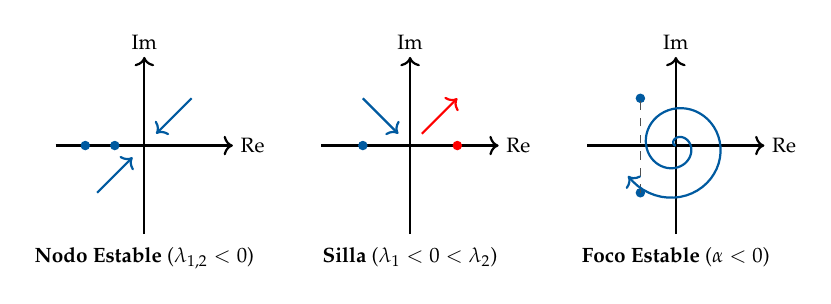
\begin{tikzpicture}[scale=0.75, every node/.style={scale=0.75}]
\begin{scope}[shift={(0,0)}]
\draw[->, thick] (-1.5,0) -- (1.5,0) node[right] {Re};
\draw[->, thick] (0,-1.5) -- (0,1.5) node[above] {Im};
\draw[themeblue, fill=themeblue] (-0.5,0) circle (2pt);
\draw[themeblue, fill=themeblue] (-1.0,0) circle (2pt);
\draw[->, themeblue, thick] (0.8,0.8) -- (0.2,0.2);
\draw[->, themeblue, thick] (-0.8,-0.8) -- (-0.2,-0.2);
\node[below] at (0,-1.6) {\textbf{Nodo Estable} ($\lambda_{1,2} < 0$)};
\end{scope}
\begin{scope}[shift={(4.5,0)}]
\draw[->, thick] (-1.5,0) -- (1.5,0) node[right] {Re};
\draw[->, thick] (0,-1.5) -- (0,1.5) node[above] {Im};
\draw[themeblue, fill=themeblue] (-0.8,0) circle (2pt);
\draw[red, fill=red] (0.8,0) circle (2pt);
\draw[->, themeblue, thick] (-0.8,0.8) -- (-0.2,0.2);
\draw[->, red, thick] (0.2,0.2) -- (0.8,0.8);
\node[below] at (0,-1.6) {\textbf{Silla} ($\lambda_1 < 0 < \lambda_2$)};
\end{scope}
\begin{scope}[shift={(9,0)}]
\draw[->, thick] (-1.5,0) -- (1.5,0) node[right] {Re};
\draw[->, thick] (0,-1.5) -- (0,1.5) node[above] {Im};
\draw[themeblue, fill=themeblue] (-0.6,0.8) circle (2pt);
\draw[themeblue, fill=themeblue] (-0.6,-0.8) circle (2pt);
\draw[dashed, themegray] (-0.6,-0.8) -- (-0.6,0.8);
\draw[->, themeblue, thick, domain=0:12, variable=\t, samples=100] plot ({-0.08*\t*cos(\t r)}, {0.08*\t*sin(\t r)});
\node[below] at (0,-1.6) {\textbf{Foco Estable} ($\alpha < 0$)};
\end{scope}
\end{tikzpicture}
\end{center}

\newpage
\cheatsheetsection{Transformadas de Laplace y Análisis Aplicado}
La Transformada de Laplace mapea ecuaciones diferenciales del dominio del tiempo a ecuaciones algebraicas en el dominio de la frecuencia (dominio $s$): $F(s) = \mathcal{L}\{f(t)\} = \int_{0}^{\infty} e^{-st}f(t)dt$.

\cheatsheetsubsection{Manejo de Condiciones Iniciales}
Las transformadas de Laplace incorporan intrínsecamente las condiciones iniciales del sistema, evitando la necesidad de resolver las constantes de integración posteriormente.
\begin{itemize}[leftmargin=*, nosep]
    \item $\mathcal{L}\{y'(t)\} = sY(s) - y(0)$
    \item $\mathcal{L}\{y''(t)\} = s^2Y(s) - sy(0) - y'(0)$
    \item $\mathcal{L}\{y^{(n)}(t)\} = s^nY(s) - s^{n-1}y(0) - \dots - y^{(n-1)}(0)$
\end{itemize}

\cheatsheetsubsection{Método de Fracciones Parciales}
Esencial para aplicar la Transformada Inversa de Laplace $\mathcal{L}^{-1}$ en funciones racionales complejas $F(s) = P(s)/Q(s)$.
\textbf{Paso 1:} Factorizar completamente el denominador $Q(s)$. \\
\textbf{Paso 2:} Construir la plantilla algebraica según los factores:
\begin{itemize}[leftmargin=*, nosep]
    \item \textbf{Lineales Distintos:} Para $(s-a)$, usar $\frac{A}{s-a}$
    \item \textbf{Lineales Repetidos:} Para $(s-a)^k$, usar $\frac{A_1}{s-a} + \frac{A_2}{(s-a)^2} + \dots + \frac{A_k}{(s-a)^k}$
    \item \textbf{Cuadráticos Irreducibles:} Para $(s^2+as+b)$, usar $\frac{As+B}{s^2+as+b}$
\end{itemize}
\textbf{Paso 3:} Resolver los coeficientes desconocidos ($A, B, \dots$) usando el método de Heaviside (cover-up) o igualando coeficientes polinomiales. \\
\textbf{Paso 4:} Aplicar la transformada inversa $\mathcal{L}^{-1}$ a cada fracción simple resultante usando la tabla.

\cheatsheetsubsection{Funciones Especiales en Sistemas Lineales}
\begin{itemize}[leftmargin=*, nosep]
    \item \textbf{Función Gamma $\Gamma(x)$:} La continuación analítica de la función factorial a números complejos/reales, definida como $\int_0^\infty t^{x-1}e^{-t}dt$. Propiedades: $\Gamma(n+1) = n!$ y $\Gamma(1/2) = \sqrt{\pi}$. Es estrictamente necesaria al calcular la transformada de Laplace de funciones con potencias fraccionarias como $t^{3/2}$.
    \item \textbf{Función Escalón de Heaviside $u_c(t)$ o $u(t-c)$:} Se evalúa como $0$ para $t < c$ y $1$ para $t \ge c$. Actúa como un interruptor matemático, muy utilizado para modelar operaciones a trozos, excitaciones retardadas y señales lógicas digitales en sistemas de control.
    \item \textbf{Función Delta de Dirac $\delta(t-c)$:} Una función generalizada (distribución) que representa un impulso infinitamente concentrado en $t=c$. Tiene un pico infinito pero integral finita $\int \delta(t-c)dt = 1$. Se usa para simular choques mecánicos instantáneos, caída de rayos o fuerzas impulsivas.
\end{itemize}

\newpage
\cheatsheetsection{Propiedades de Laplace e Identidades Operacionales}
\vspace{0.2em}
\renewcommand{\arraystretch}{1.2}
\begin{tabularx}{\linewidth}{|p{0.35\linewidth}|X|}
\hline
\textbf{Teorema / Propiedad} & \textbf{Identidad Matemática} \\ \hline
Linealidad & $\mathcal{L}\{af(t) + bg(t)\} = aF(s) + bG(s)$ \\ \hline
Primer Teorema de Traslación & $\mathcal{L}\{e^{at}f(t)\} = F(s-a)$ \\ \hline
Segundo Teorema de Traslación & $\mathcal{L}\{u_c(t)f(t-c)\} = e^{-cs}F(s)$ \\ \hline
Transformada de una Integral & $\mathcal{L}\{\int_0^t f(\tau)d\tau\} = \frac{F(s)}{s}$ \\ \hline
Multiplicación por $t^n$ & $\mathcal{L}\{t^n f(t)\} = (-1)^n \frac{d^n}{ds^n}F(s)$ \\ \hline
División por $t$ & $\mathcal{L}\{\frac{f(t)}{t}\} = \int_s^\infty F(u)du$ \\ \hline
Teorema de Convolución & $\mathcal{L}\{(f * g)(t)\} = F(s)G(s)$ \\ \hline
Función Periódica ($T$) & $\mathcal{L}\{f(t)\} = \frac{1}{1-e^{-sT}} \int_0^T e^{-st}f(t)dt$ \\ \hline
\end{tabularx}

\cheatsheetsection{Trampas y Errores Comunes en Laplace}
\begin{itemize}[leftmargin=*, nosep]
    \item \textbf{Violación de Linealidad en la Multiplicación:} Asumir $\mathcal{L}\{f(t)g(t)\} = F(s)G(s)$. Esto es falso; la multiplicación en el dominio del tiempo requiere una convolución compleja en el dominio $s$.
    \item \textbf{Traslación Temporal Incorrecta (Inversa):} Olvidar desplazar el argumento temporal de la función al regresar de una exponencial en el dominio $s$. $\mathcal{L}^{-1}\{e^{-cs}F(s)\} = u_c(t)f(t-c)$, no $u_c(t)f(t)$.
    \item \textbf{Numerador Cuadrático Incompleto:} Establecer una fracción parcial para una cuadrática irreducible como $s^2+4$ usando solo $A$ en el numerador en lugar de $As+B$.
\end{itemize}

\clearpage 

\begingroup
\large
\renewcommand{\arraystretch}{1.4}

\cheatsheetsection{Tabla de Transformadas de Laplace Comunes}
\vspace{0.5em}

\begin{tabularx}{\linewidth}{|p{0.45\linewidth}|X|}
\hline
\textbf{Función $f(t) = \mathcal{L}^{-1}\{F(s)\}$} & \textbf{Transformada $F(s) = \mathcal{L}\{f(t)\}$} \\ \hline
$1$ & $\frac{1}{s}$ \\ \hline
$t^n \quad (n = 1,2,3,\dots)$ & $\frac{n!}{s^{n+1}}$ \\ \hline
$t^p \quad (p > -1)$ & $\frac{\Gamma(p+1)}{s^{p+1}}$ \\ \hline
$\sqrt{t}$ & $\frac{\sqrt{\pi}}{2s^{3/2}}$ \\ \hline
$t^{n-1/2} \quad (n = 1,2,\dots)$ & $\frac{1 \cdot 3 \dots (2n-1)\sqrt{\pi}}{2^n s^{n+1/2}}$ \\ \hline
$e^{at}$ & $\frac{1}{s-a}$ \\ \hline
$t^n e^{at}$ & $\frac{n!}{(s-a)^{n+1}}$ \\ \hline
$\sin(at)$ & $\frac{a}{s^2+a^2}$ \\ \hline
$\cos(at)$ & $\frac{s}{s^2+a^2}$ \\ \hline
$\sinh(at)$ & $\frac{a}{s^2-a^2}$ \\ \hline
$\cosh(at)$ & $\frac{s}{s^2-a^2}$ \\ \hline
$t \sin(at)$ & $\frac{2as}{(s^2+a^2)^2}$ \\ \hline
$t \cos(at)$ & $\frac{s^2-a^2}{(s^2+a^2)^2}$ \\ \hline
$t \sinh(at)$ & $\frac{2as}{(s^2-a^2)^2}$ \\ \hline
$t \cosh(at)$ & $\frac{s^2+a^2}{(s^2-a^2)^2}$ \\ \hline
$e^{at}\sin(bt)$ & $\frac{b}{(s-a)^2+b^2}$ \\ \hline
$e^{at}\cos(bt)$ & $\frac{s-a}{(s-a)^2+b^2}$ \\ \hline
$e^{at}\sinh(bt)$ & $\frac{b}{(s-a)^2-b^2}$ \\ \hline
$e^{at}\cosh(bt)$ & $\frac{s-a}{(s-a)^2-b^2}$ \\ \hline
\end{tabularx}

\newpage

\cheatsheetsection{Tabla de Transformadas de Laplace Comunes}
\vspace{0.5em}

\begin{tabularx}{\linewidth}{|p{0.45\linewidth}|X|}
\hline
\textbf{Función $f(t) = \mathcal{L}^{-1}\{F(s)\}$} & \textbf{Transformada $F(s) = \mathcal{L}\{f(t)\}$} \\ \hline
$\sin(at) - at \cos(at)$ & $\frac{2a^3}{(s^2+a^2)^2}$ \\ \hline
$\sin(at) + at \cos(at)$ & $\frac{2as^2}{(s^2+a^2)^2}$ \\ \hline
$\cos(at) - at \sin(at)$ & $\frac{s(s^2-a^2)}{(s^2+a^2)^2}$ \\ \hline
$\cos(at) + at \sin(at)$ & $\frac{s(s^2+3a^2)}{(s^2+a^2)^2}$ \\ \hline
$u_c(t)$ o $u(t-c)$ & $\frac{e^{-cs}}{s}$ \\ \hline
$\delta(t-c)$ & $e^{-cs}$ \\ \hline
$1 - \cos(at)$ & $\frac{a^2}{s(s^2+a^2)}$ \\ \hline
$at - \sin(at)$ & $\frac{a^3}{s^2(s^2+a^2)}$ \\ \hline
$\frac{1}{a-b}(e^{at} - e^{bt})$ & $\frac{1}{(s-a)(s-b)}$ \\ \hline
$\frac{1}{a-b}(a e^{at} - b e^{bt})$ & $\frac{s}{(s-a)(s-b)}$ \\ \hline
$\frac{1}{t}\sin(at)$ & $\arctan\left(\frac{a}{s}\right)$ \\ \hline
$\frac{1}{t}(1 - \cos(at))$ & $\frac{1}{2}\ln\left(\frac{s^2+a^2}{s^2}\right)$ \\ \hline
$\frac{1}{t}(1 - e^{-at})$ & $\ln\left(\frac{s+a}{s}\right)$ \\ \hline
$J_0(at)$ (Función de Bessel) & $\frac{1}{\sqrt{s^2+a^2}}$ \\ \hline
$J_0(2\sqrt{kt})$ & $\frac{1}{s}e^{-k/s}$ \\ \hline
$\frac{1}{\sqrt{\pi t}}e^{-a^2/4t}$ & $\frac{1}{\sqrt{s}}e^{-a\sqrt{s}}$ \\ \hline
$\frac{a}{2\sqrt{\pi t^3}}e^{-a^2/4t}$ & $e^{-a\sqrt{s}}$ \\ \hline
$e^{at} - at - 1$ & $\frac{a^2}{s^2(s-a)}$ \\ \hline
$f(t) * g(t)$ (Convolución) & $F(s)G(s)$ \\ \hline
\end{tabularx}
\endgroup

\clearpage
\onecolumn

\cheatsheetsection{Árbol de Decisión de Estrategias de Solución para EDOs}
\vspace{1em}

\begin{center}
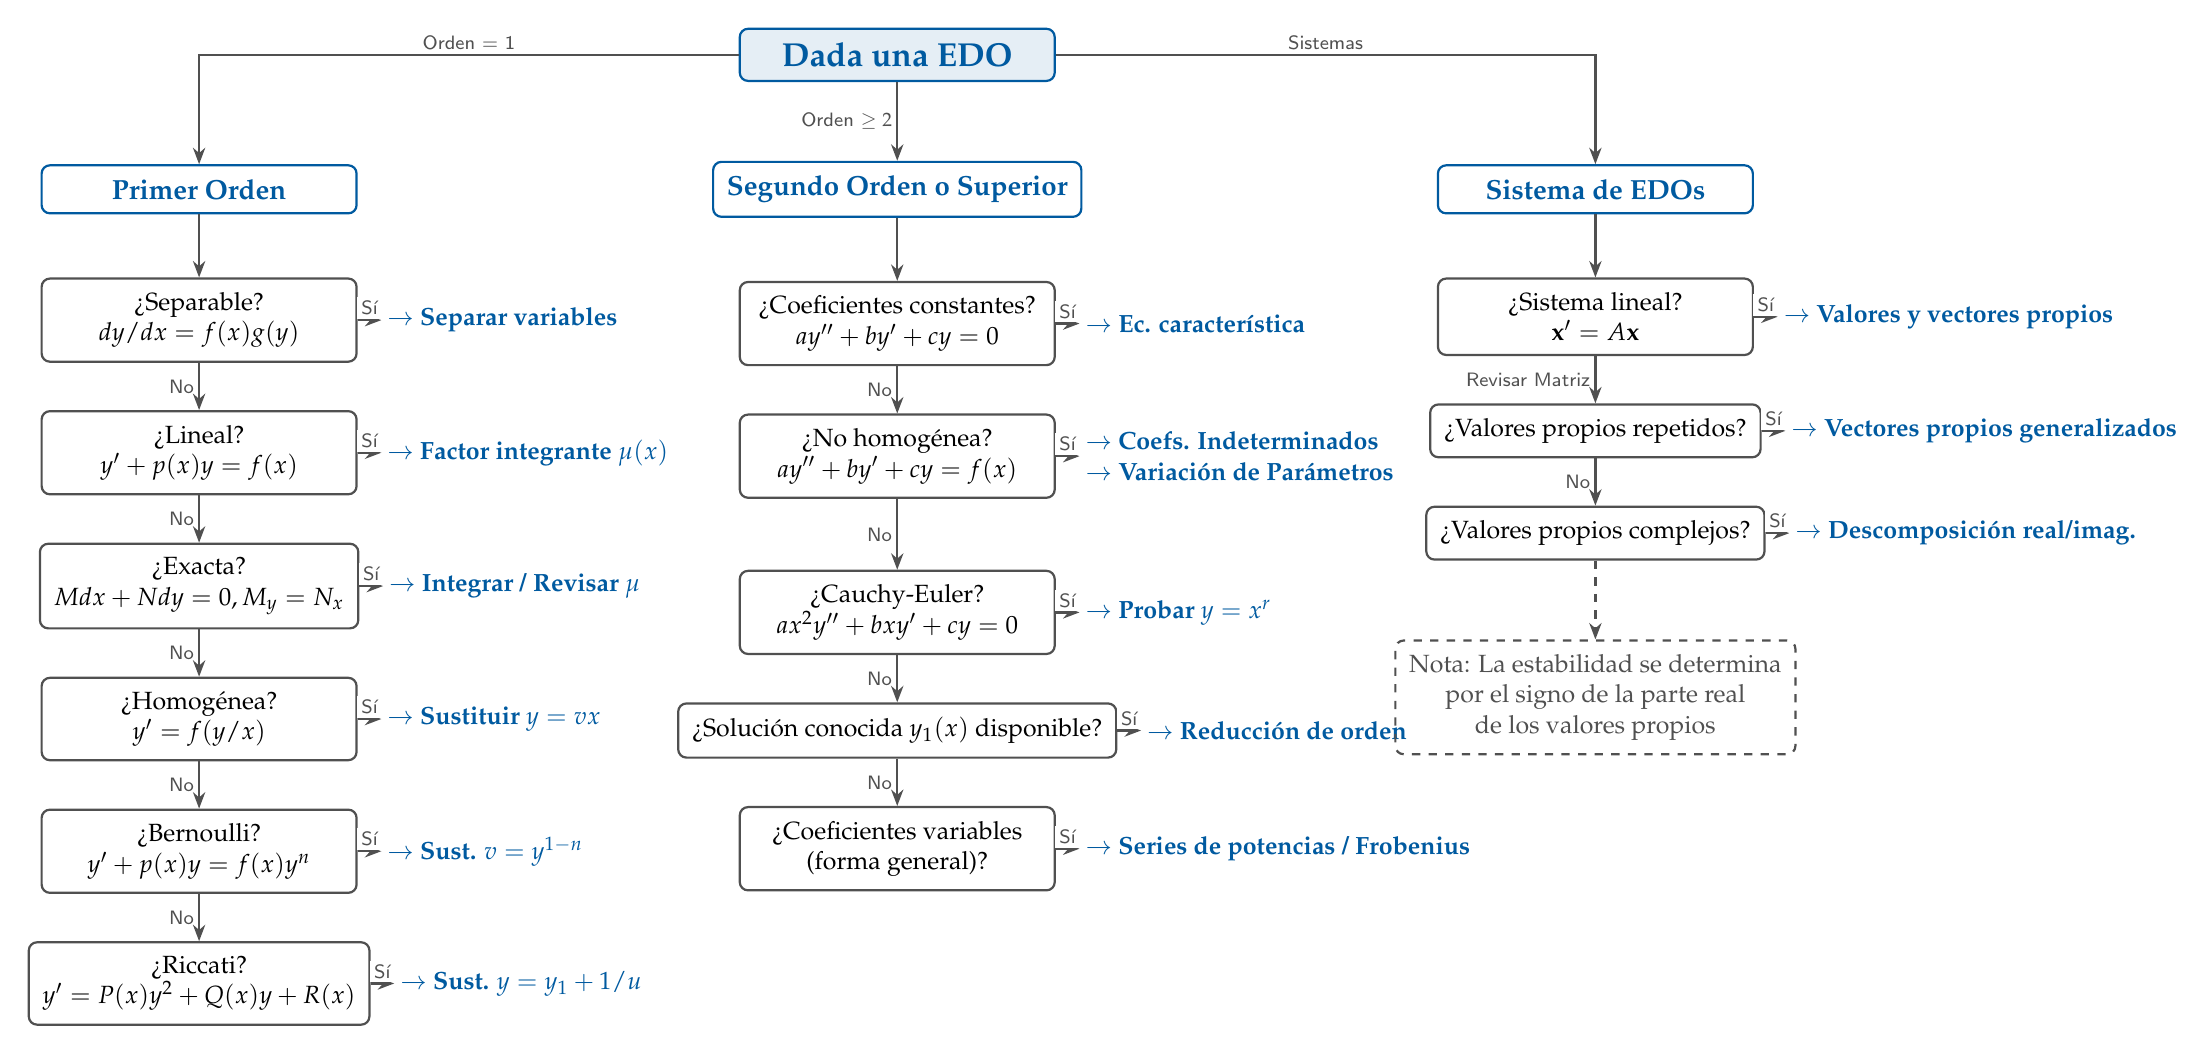
\begin{tikzpicture}[
    node distance=0.6cm and 0.8cm,
    base/.style={rectangle, rounded corners=3pt, draw=themegray, thick, align=center, font=\small, inner sep=5pt},
    root/.style={base, draw=themeblue, fill=themeblue!10, text=themeblue, font=\large\bfseries, minimum width=4cm},
    category/.style={base, draw=themeblue, fill=white, text=themeblue, font=\normalsize\bfseries, minimum width=4cm},
    decision/.style={base, fill=white, minimum width=4cm, text=black},
    method/.style={rectangle, align=left, text=themeblue, font=\small\bfseries, inner sep=2pt},
    line/.style={draw=themegray, thick, -{Stealth[scale=0.9]}},
    label/.style={font=\scriptsize\sffamily, text=themegray, fill=white, inner sep=1.5pt}
]

\node[root] (start) {Dada una EDO};

\node[category, below=1cm of start] (second) {Segundo Orden o Superior};
\node[category, left=4.5cm of second] (first) {Primer Orden};
\node[category, right=4.5cm of second] (system) {Sistema de EDOs};

\draw[line] (start) -| node[label, near start, above] {Orden = 1} (first);
\draw[line] (start) -- node[label, fill=none, left] {Orden $\ge 2$} (second);
\draw[line] (start) -| node[label, near start, above] {Sistemas} (system);

\node[decision, below=0.8cm of first] (sep) {¿Separable?\\$dy/dx = f(x)g(y)$};
\node[method, right=0.3cm of sep] (m_sep) {$\rightarrow$ Separar variables};

\node[decision, below=0.6cm of sep] (lin) {¿Lineal?\\$y' + p(x)y = f(x)$};
\node[method, right=0.3cm of lin] (m_lin) {$\rightarrow$ Factor integrante $\mu(x)$};

\node[decision, below=0.6cm of lin] (exact) {¿Exacta?\\$M dx + N dy = 0, M_y=N_x$};
\node[method, right=0.3cm of exact] (m_exact) {$\rightarrow$ Integrar / Revisar $\mu$};

\node[decision, below=0.6cm of exact] (homo) {¿Homogénea?\\$y' = f(y/x)$};
\node[method, right=0.3cm of homo] (m_homo) {$\rightarrow$ Sustituir $y = vx$};

\node[decision, below=0.6cm of homo] (ber) {¿Bernoulli?\\$y' + p(x)y = f(x)y^n$};
\node[method, right=0.3cm of ber] (m_ber) {$\rightarrow$ Sust. $v = y^{1-n}$};

\node[decision, below=0.6cm of ber] (ric) {¿Riccati?\\$y' = P(x)y^2 + Q(x)y + R(x)$};
\node[method, right=0.3cm of ric] (m_ric) {$\rightarrow$ Sust. $y = y_1 + 1/u$};

\draw[line] (first) -- (sep);
\draw[line] (sep) -- node[label, above] {Sí} (m_sep);
\draw[line] (sep) -- node[label, fill=none, left] {No} (lin);
\draw[line] (lin) -- node[label, above] {Sí} (m_lin);
\draw[line] (lin) -- node[label, fill=none, left] {No} (exact);
\draw[line] (exact) -- node[label, above] {Sí} (m_exact);
\draw[line] (exact) -- node[label, fill=none, left] {No} (homo);
\draw[line] (homo) -- node[label, above] {Sí} (m_homo);
\draw[line] (homo) -- node[label, fill=none, left] {No} (ber);
\draw[line] (ber) -- node[label, above] {Sí} (m_ber);
\draw[line] (ber) -- node[label, fill=none, left] {No} (ric);
\draw[line] (ric) -- node[label, above] {Sí} (m_ric);

\node[decision, below=0.8cm of second] (const) {¿Coeficientes constantes?\\$ay''+by'+cy=0$};
\node[method, right=0.3cm of const] (m_const) {$\rightarrow$ Ec. característica};

\node[decision, below=0.6cm of const] (nonhomo) {¿No homogénea?\\$ay''+by'+cy=f(x)$};
\node[method, right=0.3cm of nonhomo, align=left] (m_nonhomo) {$\rightarrow$ Coefs. Indeterminados\\$\rightarrow$ Variación de Parámetros};

\node[decision, below=0.9cm of nonhomo] (euler) {¿Cauchy-Euler?\\$ax^2y''+bxy'+cy=0$};
\node[method, right=0.3cm of euler] (m_euler) {$\rightarrow$ Probar $y = x^r$};

\node[decision, below=0.6cm of euler] (known) {¿Solución conocida $y_1(x)$ disponible?};
\node[method, right=0.3cm of known] (m_known) {$\rightarrow$ Reducción de orden};

\node[decision, below=0.6cm of known] (var) {¿Coeficientes variables\\(forma general)?};
\node[method, right=0.3cm of var] (m_var) {$\rightarrow$ Series de potencias / Frobenius};

\draw[line] (second) -- (const);
\draw[line] (const) -- node[label, above] {Sí} (m_const);
\draw[line] (const) -- node[label, fill=none, left] {No} (nonhomo);
\draw[line] (nonhomo) -- node[label, above] {Sí} (m_nonhomo);
\draw[line] (nonhomo) -- node[label, fill=none, left] {No} (euler);
\draw[line] (euler) -- node[label, above] {Sí} (m_euler);
\draw[line] (euler) -- node[label, fill=none, left] {No} (known);
\draw[line] (known) -- node[label, above] {Sí} (m_known);
\draw[line] (known) -- node[label, fill=none, left] {No} (var);
\draw[line] (var) -- node[label, above] {Sí} (m_var);


\node[decision, below=0.8cm of system] (linsys) {¿Sistema lineal?\\$\mathbf{x}' = A\mathbf{x}$};
\node[method, right=0.3cm of linsys] (m_linsys) {$\rightarrow$ Valores y vectores propios};

\node[decision, below=0.6cm of linsys] (rep) {¿Valores propios repetidos?};
\node[method, right=0.3cm of rep] (m_rep) {$\rightarrow$ Vectores propios generalizados};

\node[decision, below=0.6cm of rep] (comp) {¿Valores propios complejos?};
\node[method, right=0.3cm of comp] (m_comp) {$\rightarrow$ Descomposición real/imag.};

\node[base, draw=themegray, dashed, below=1cm of comp, text=themegray] (stab) {Nota: La estabilidad se determina\\por el signo de la parte real\\de los valores propios};

\draw[line] (system) -- (linsys);
\draw[line] (linsys) -- node[label, above] {Sí} (m_linsys);
\draw[line] (linsys) -- node[label, fill=none, left] {Revisar Matriz} (rep);
\draw[line] (rep) -- node[label, above] {Sí} (m_rep);
\draw[line] (rep) -- node[label, fill=none, left] {No} (comp);
\draw[line] (comp) -- node[label, above] {Sí} (m_comp);

\draw[line, dashed, draw=themegray] (comp) -- (stab);

\end{tikzpicture}
\end{center}

\end{document}